\documentclass[a4paper,12pt]{article}

\usepackage[utf8]{inputenc}
\usepackage{geometry}
\usepackage{graphicx}
\graphicspath{{Figures/}}
\usepackage{mathptmx}
\usepackage{setspace}
\usepackage{titlesec}
\usepackage{parskip}
\usepackage{enumitem}
\usepackage{indentfirst}
\usepackage{listings}
\usepackage{xcolor}
\usepackage{hyperref}
\usepackage{xurl}
\usepackage{microtype}
\usepackage{float}
\setlength{\emergencystretch}{1em}
\sloppy

\lstset{
    breaklines=true,
    postbreak=\mbox{\textcolor{red}{$\hookrightarrow$}\space},
}

\setlength{\parindent}{1em}

\definecolor{dkgreen}{rgb}{0,0.6,0}
\definecolor{gray}{rgb}{0.5,0.5,0.5}
\definecolor{mauve}{rgb}{0.58,0,0.82}
\definecolor{dkblue}{rgb}{0,0,0.5}
\definecolor{lightblue}{rgb}{0,0.5,0.8}
\definecolor{darkred}{rgb}{0.6,0,0}
\definecolor{backcolour}{rgb}{0.97,0.97,0.97}

\lstdefinestyle{javastyle}{
    language=Java,
    backgroundcolor=\color{backcolour},   
    commentstyle=\color{dkgreen}\itshape,
    keywordstyle=\color{dkblue}\bfseries,
    stringstyle=\color{mauve},
    basicstyle=\ttfamily\footnotesize,
    breakatwhitespace=false,         
    breaklines=true,                 
    captionpos=b,                    
    keepspaces=true,                 
    numbers=left,                    
    numbersep=5pt,                  
    showspaces=false,                
    showstringspaces=false,
    showtabs=false,                  
    tabsize=4,
    frame=lines,
    rulecolor=\color{gray},
    moredelim=[s][\color{orange}]{@}{\ },
}

\lstdefinestyle{xmlstyle}{
    language=XML,
    backgroundcolor=\color{backcolour},
    basicstyle=\ttfamily\footnotesize,
    morekeywords={xmlns,version,type,scope,groupId,artifactId,dependencies,dependency,project,modelVersion,build,plugins,plugin,configuration,source,target},
    keywordstyle=\color{darkred}\bfseries,
    commentstyle=\color{dkgreen}\itshape,
    stringstyle=\color{dkblue},
    tagstyle=\color{darkred},
    breaklines=true,
    numbers=left,
    numbersep=5pt,
    tabsize=2,
    frame=lines
}

\geometry{
    top=3cm,
    left=4cm,
    right=3cm,
    bottom=3cm
}

\renewcommand{\thesection}{\Alph{section}} 

\renewcommand{\thesubsection}{\thesection.\arabic{subsection}}

\titleformat{\section}
  {\normalfont\Large\bfseries}
  {\thesection.}
  {1em}
  {}

\begin{document}

\begin{titlepage}
    \centering
    \onehalfspacing

    {\fontsize{14}{17}\selectfont \textbf{LAPORAN PRAKTIKUM}} \\[0.2cm]
    {\fontsize{16}{19}\selectfont \textbf{PRAKTIKUM PENGUJIAN PERANGKAT LUNAK}} \\[0.5cm]
    {\fontsize{14}{17}\selectfont \textbf{PERTEMUAN 5}} \\[0.2cm]
    {\fontsize{14}{17}\selectfont \textbf{Skenario Pengujian dan Pelaporan Bug}}
    
    \vfill
    
\includegraphics[width=6cm]{Figures/UGM.png} 
    \vfill
    
    {\large Disusun Oleh:} \\[0.5cm]
    
    \begin{tabular}{l c l} 
        Nama & : & Abdullah Afif Habiburrohman \\
        NIM  & : & 537611/SV/24441 \\
        Kelas & : & BB / B2 \\
        Dosen & : & Divi Galih Prasetyo Putri, S.Kom., M.Kom., Ph.D.
    \end{tabular}
    
    \vfill
    
    {\fontsize{12}{14}\selectfont \textbf{
        PROGRAM STUDI SARJANA TERAPAN \\ 
        TEKNOLOGI REKAYASA PERANGKAT LUNAK \\
        DEPARTEMEN TEKNIK ELEKTRO DAN INFORMATIKA \\
        SEKOLAH VOKASI \\
        UNIVERSITAS GADJAH MADA \\
        YOGYAKARTA \\
        2026
    }}
    
\end{titlepage}

\newpage

\section{Hasil dan Pembahasan}
Laporan praktikum ini berisi langkah-langkah penggunaan \url{qase.io} untuk membuat skenario pengujian dan pelaporan bug. Berikut adalah tugas-tugas yang harus dilakukan:

\begin{enumerate}
    \item Masuk ke website QASE.io dan buatlah akun (disarankan akun vang free)
    \item Login menggunakan akun yang baru dibuat
    \item Buat Project baru dengan memilih menu "Create new project"
    \item Buat project TRPL-Commerce pada QASE.io dan kasus uji (positif dan negatif) untuk user story dan acceptance criteria pada studi kasus provek PAD (tiap anggota kelompok membuat kasus uji untuk user story yang berbeda)!
    \item Lakukan pengujian berdasarkan kasus uji yang telah dibuat!
    \item Buatlah bug report untuk bug yang ditemukan. (\url{https://help.qase.io/en/articles/5563710-defects})
    \item Laporkan dalam bentuk langkah-langkah beserta screenshot tampilan QASE.io.
\end{enumerate}

Berikut adalah hasil dari setiap langkah yang telah dilakukan:
\subsection{Buat akun dan login}
Mahasiswa mendaftar menggunakan akun google UGM. Setelah mendaftar, mahasiswa otomatis terdaftar ke Qase Business tanpa perlu melakukan setting tambahan. Setelah berhasil mendaftar, mahasiswa langsung masuk ke dashboard Qase.io. Berikut adalah gambar profil dari mahasiswa:

\begin{figure}[H]
    \centering
    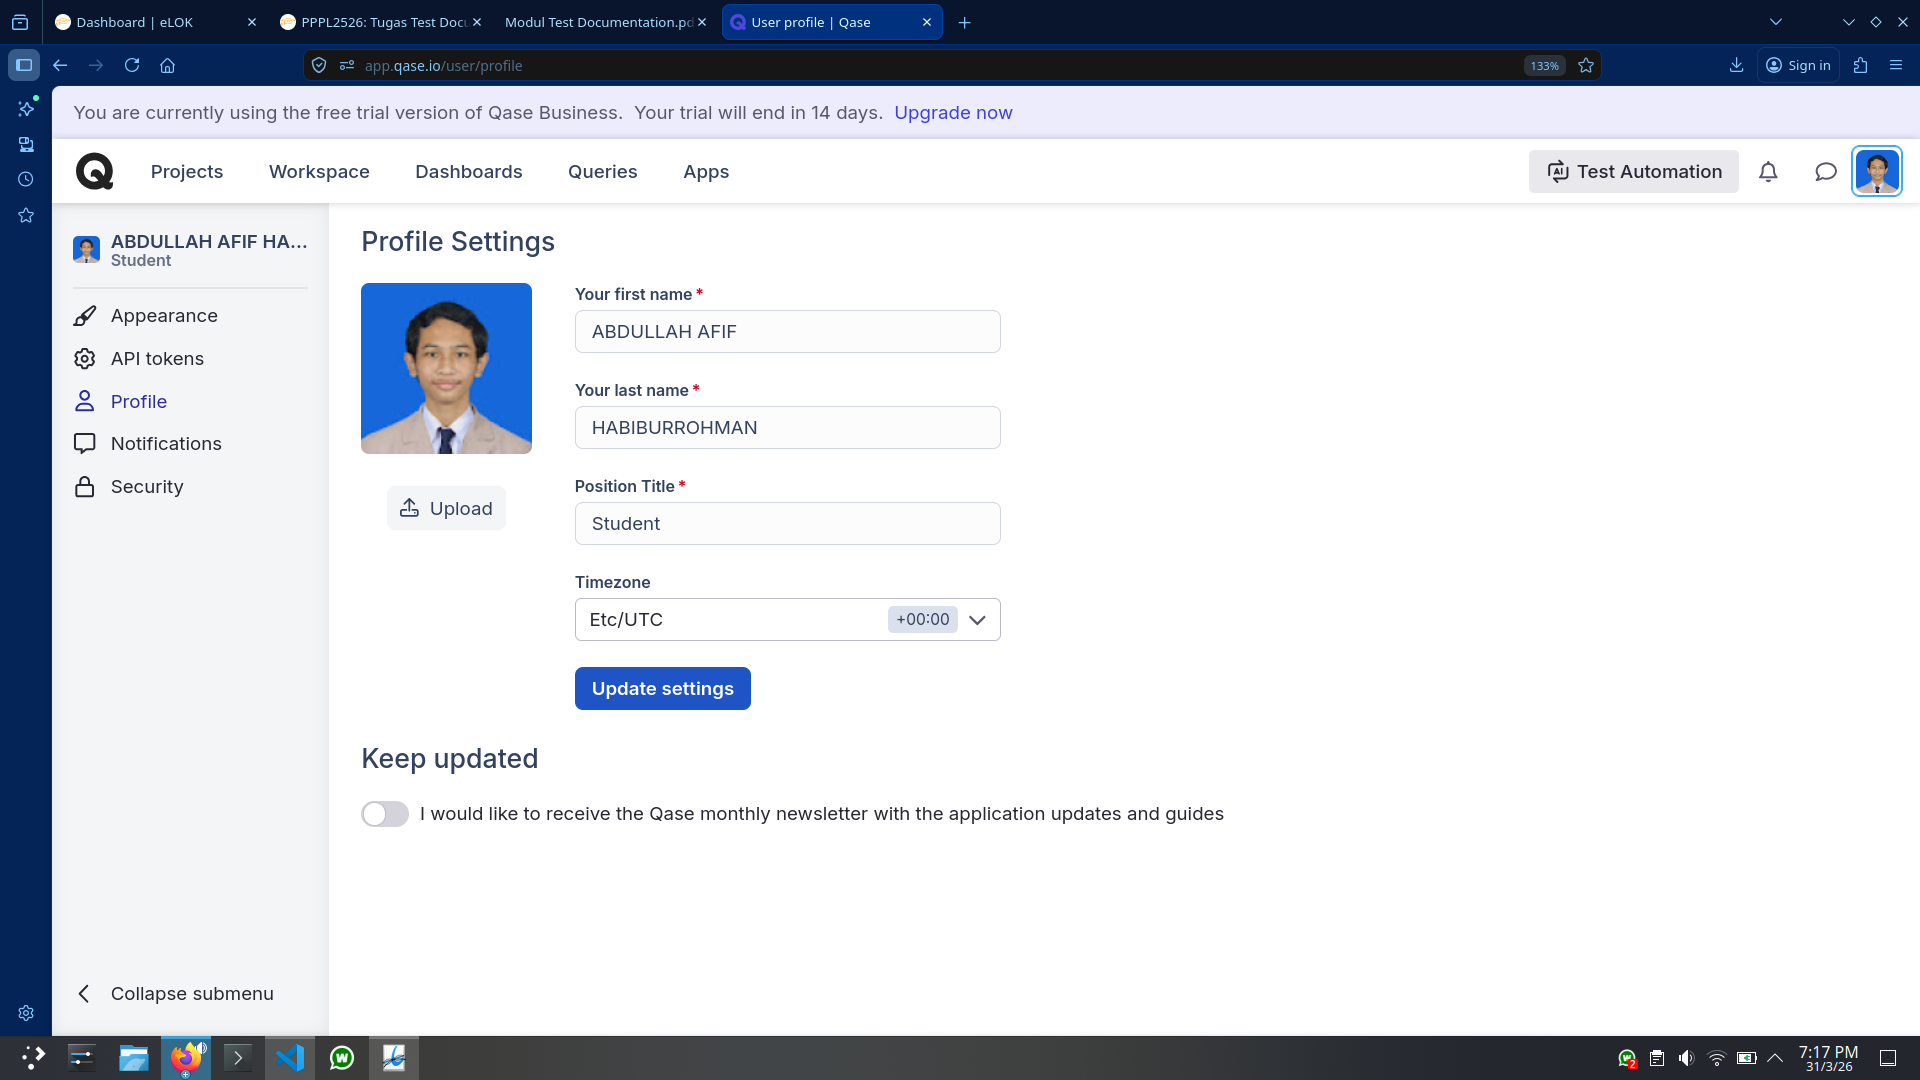
\includegraphics[width=0.8\textwidth]{image.png}
    \caption{Profil Mahasiswa}
    \label{fig:profil}
\end{figure}

\subsection{Buat project baru}
Mahasiswa lalu pergi ke halaman dashboard. Pada halaman dashboard, mahasiswa memilih menu "Create new project". Setelah itu, mahasiswa mengisi nama project dengan "TRPL-Commerce". Setelah itu, mahasiswa menekan tombol "Create" untuk membuat project baru. Berikut adalah gambar dari halaman create project:

\begin{figure}[H]
    \centering
    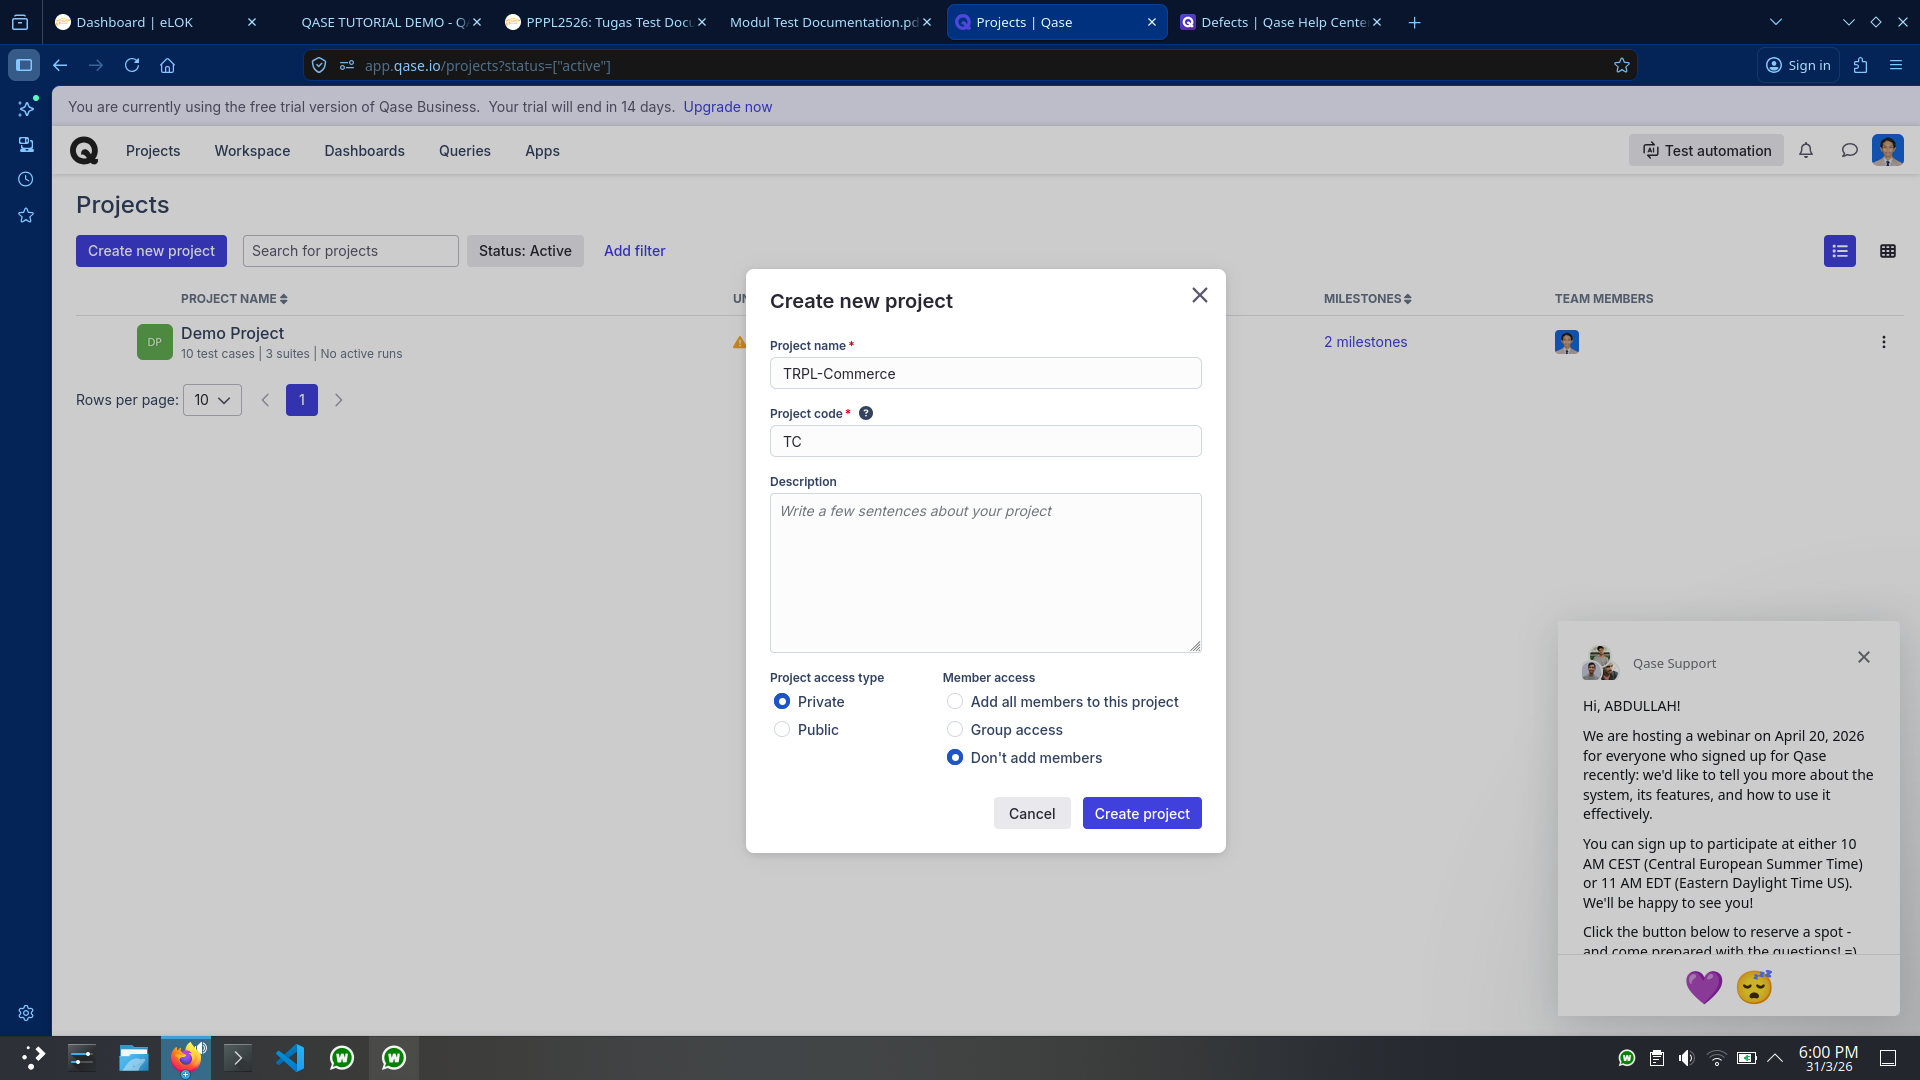
\includegraphics[width=0.8\textwidth]{Screenshot_20260331_180048.png}
    \caption{Halaman Create Project}
    \label{fig:create_project}
\end{figure}

\subsection{Buat test case}
Mahasiswa membuat suite baru dengan nama "Adding A Fleet". Setelah itu, mahasiswa membuat dua test case, yaitu "Positive - Valid Data" dan "Negative - Invalid Data". Kemudian, mahasiswa mengisi field-field yang diperlukan untuk setiap test case. Berikut adalah gambar langkah-langkah yang dilakukan:

\begin{figure}[H]
    \centering
    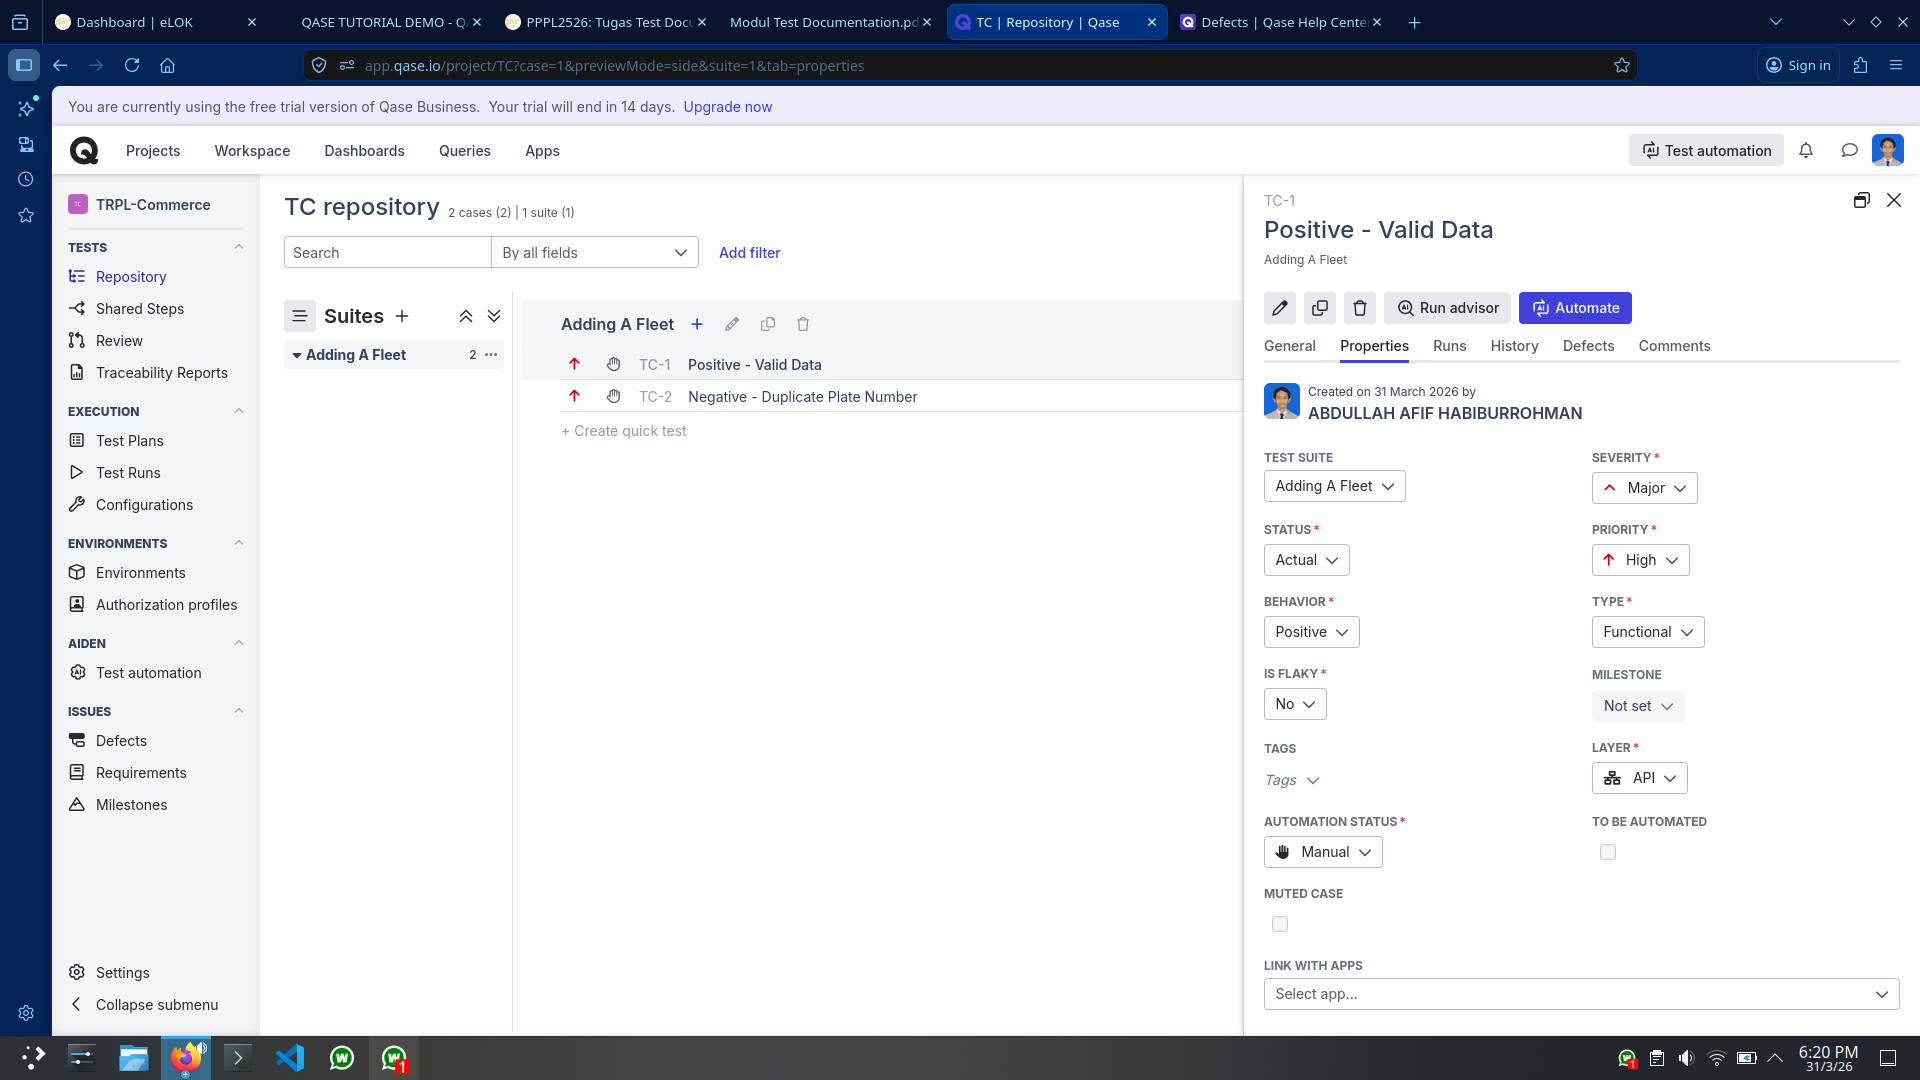
\includegraphics[width=0.8\textwidth]{Screenshot_20260331_182012.png}
    \caption{Positive - Valid Data}
    \label{fig:test_case}
\end{figure}

\begin{figure}[H]
    \centering
    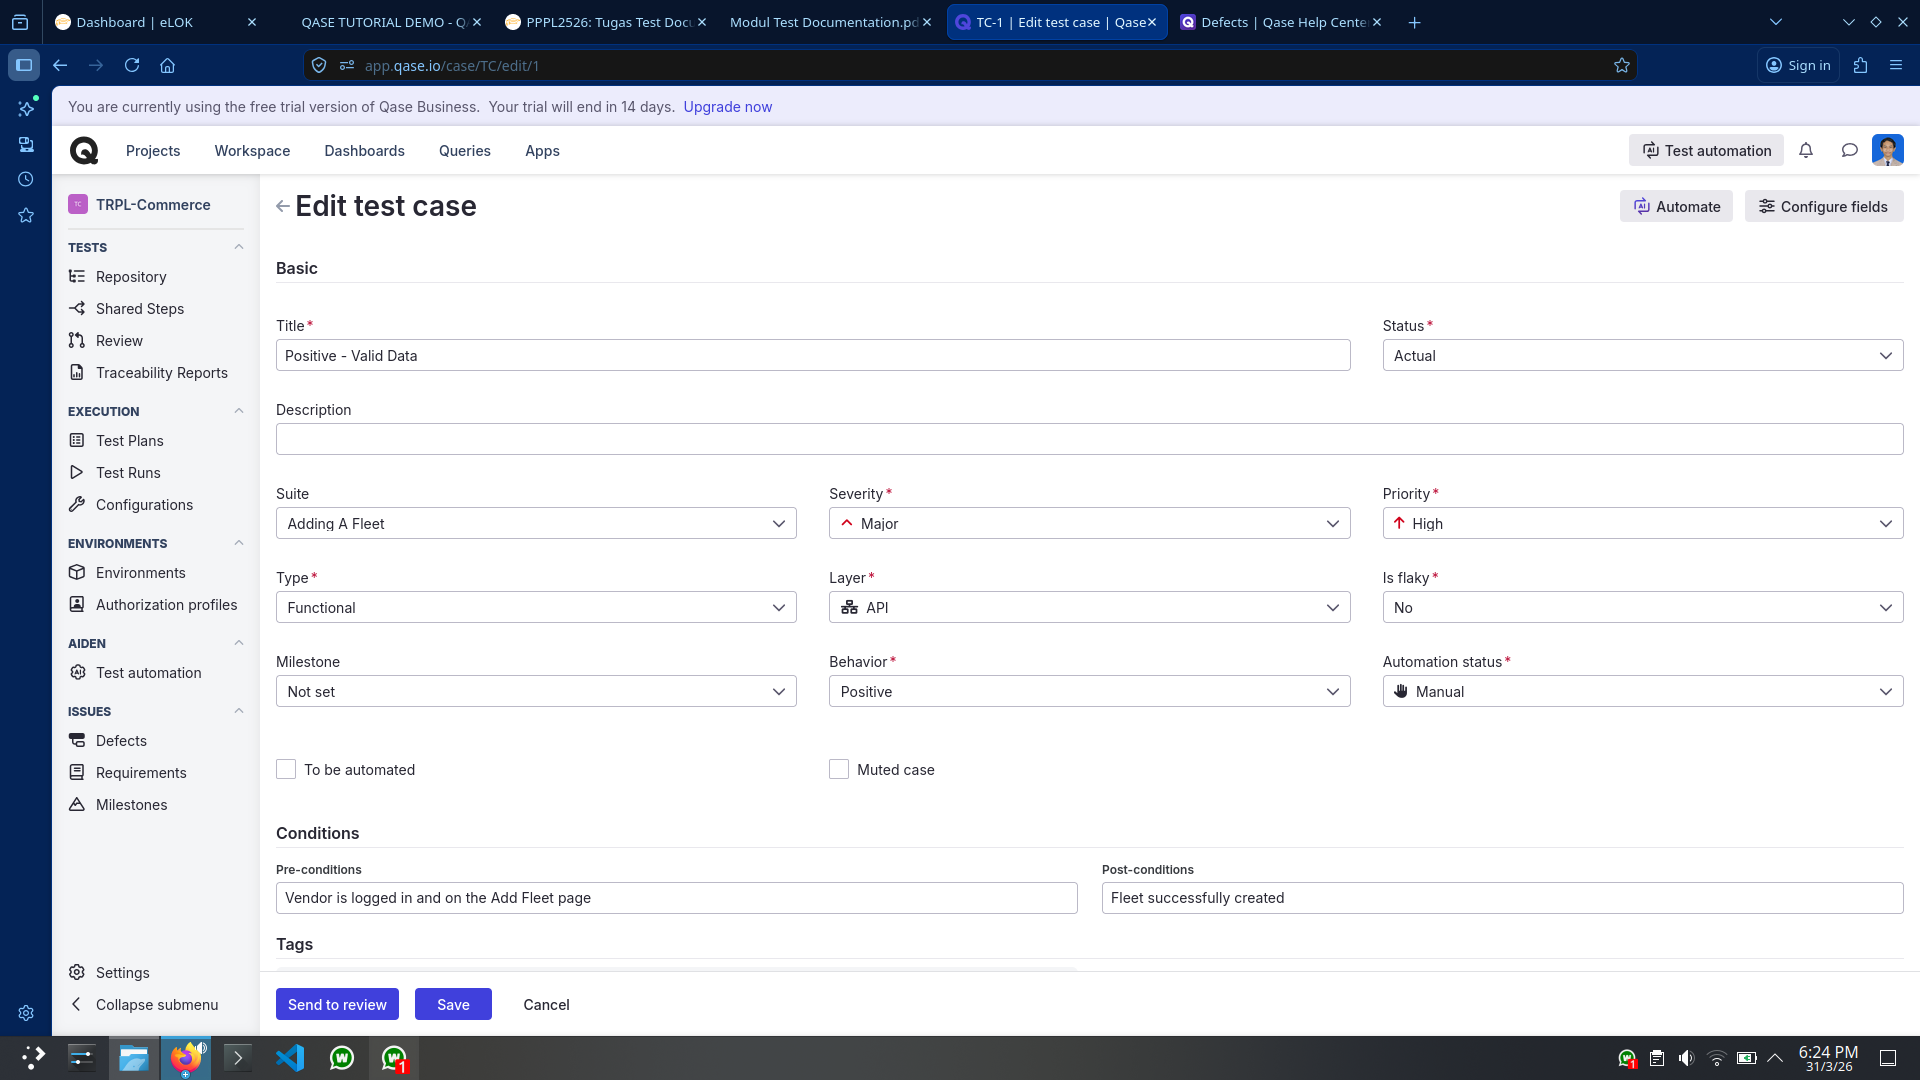
\includegraphics[width=0.8\textwidth]{Screenshot_20260331_182407.png}
    \caption{Positive - Valid Data Extended}
    \label{fig:test_case1}
\end{figure}

Untuk data "Negative - Invalid Data", mahasiswa mengisi field-field berlawanan dengan data "Positive - Valid Data".

\subsection{Lakukan pengujian}
Kemudian, mahasiswa membuat pengujian baru dengan melakukan selection ke kedua test case. Kemudian pada opsi di atas, terdapat gambar untuk run. Mahasiswa diberikan popup berisi "New test run". Mahasiswa mengisi data-data pada text field yang tersedia. Setelah itu, mahasiswa menekan tombol "Start run". Berikut adalah gambar langkah-langkah yang mahasiswa lakukan:

\begin{figure}[H]
    \centering
    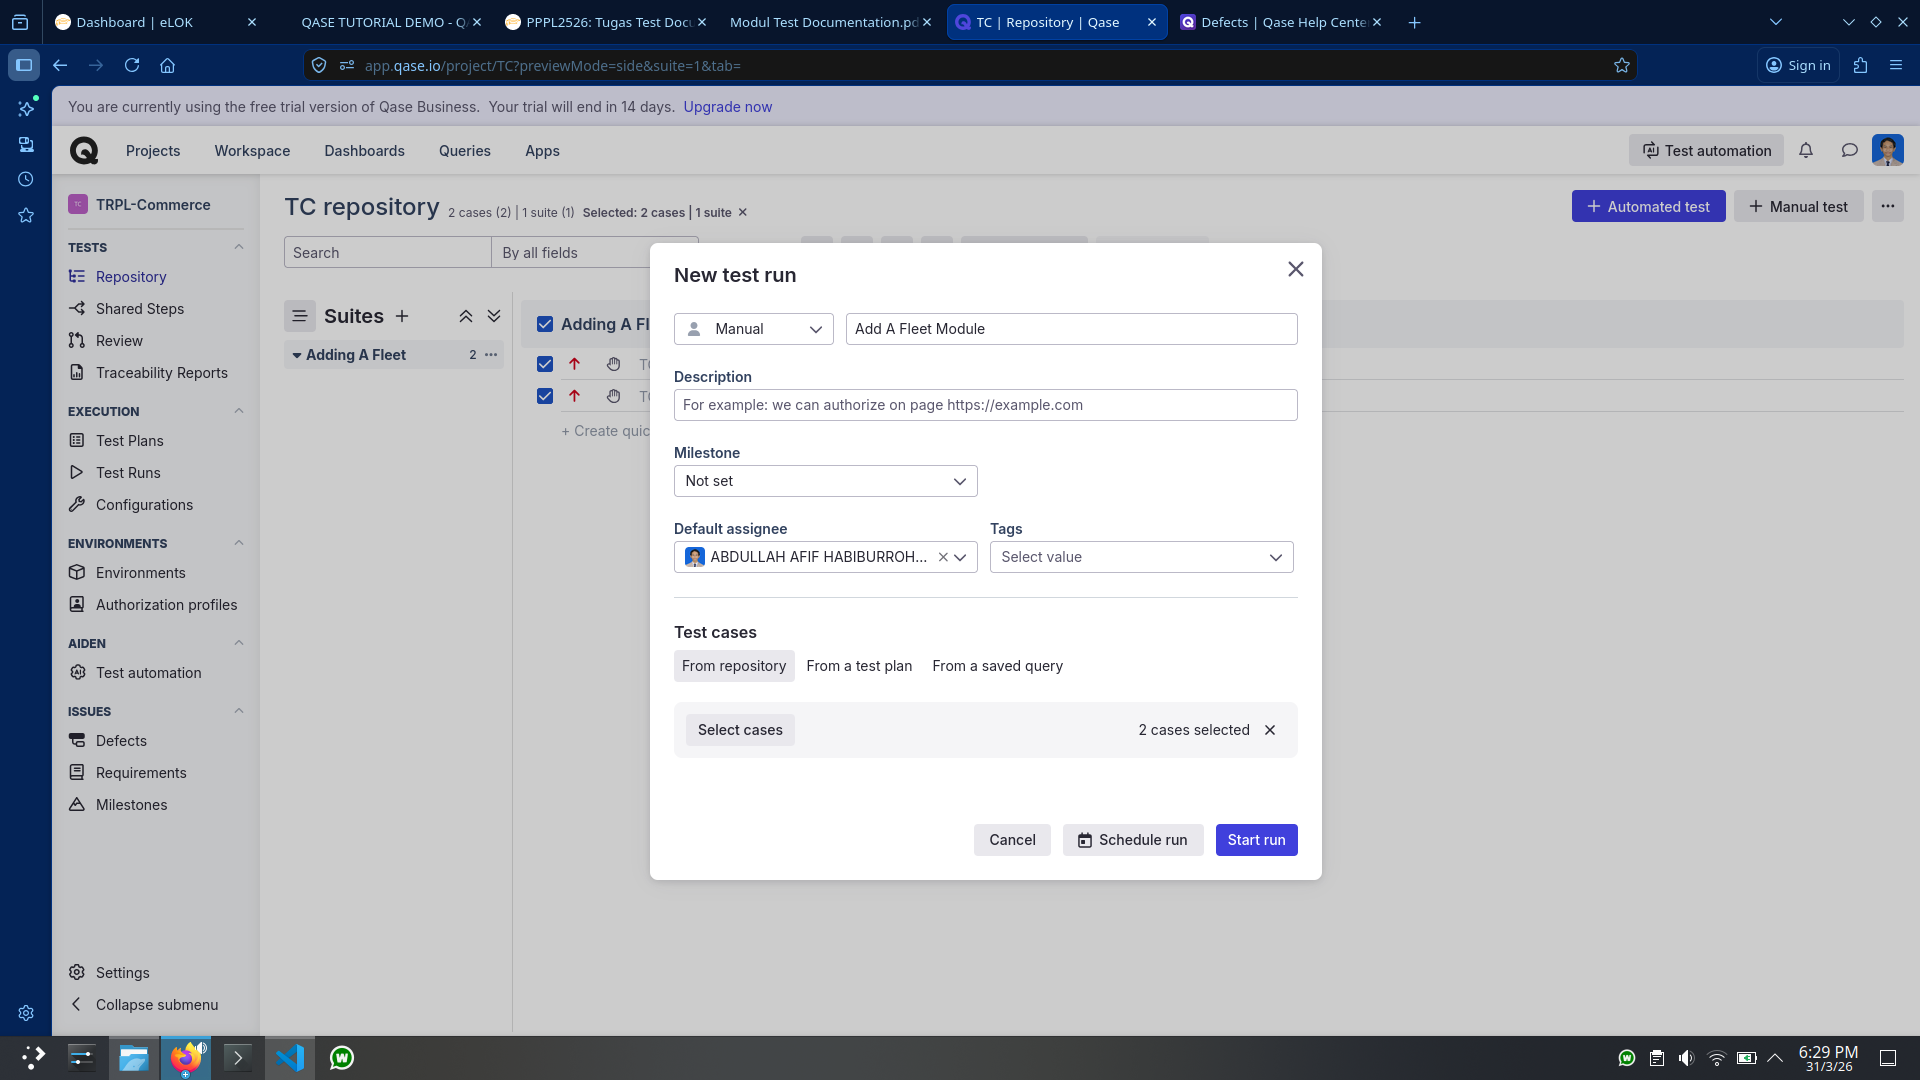
\includegraphics[width=0.8\textwidth]{Screenshot_20260331_182913.png}
    \caption{New Test Run}
    \label{fig:test_run}
\end{figure}

\begin{figure}[H]
    \centering
    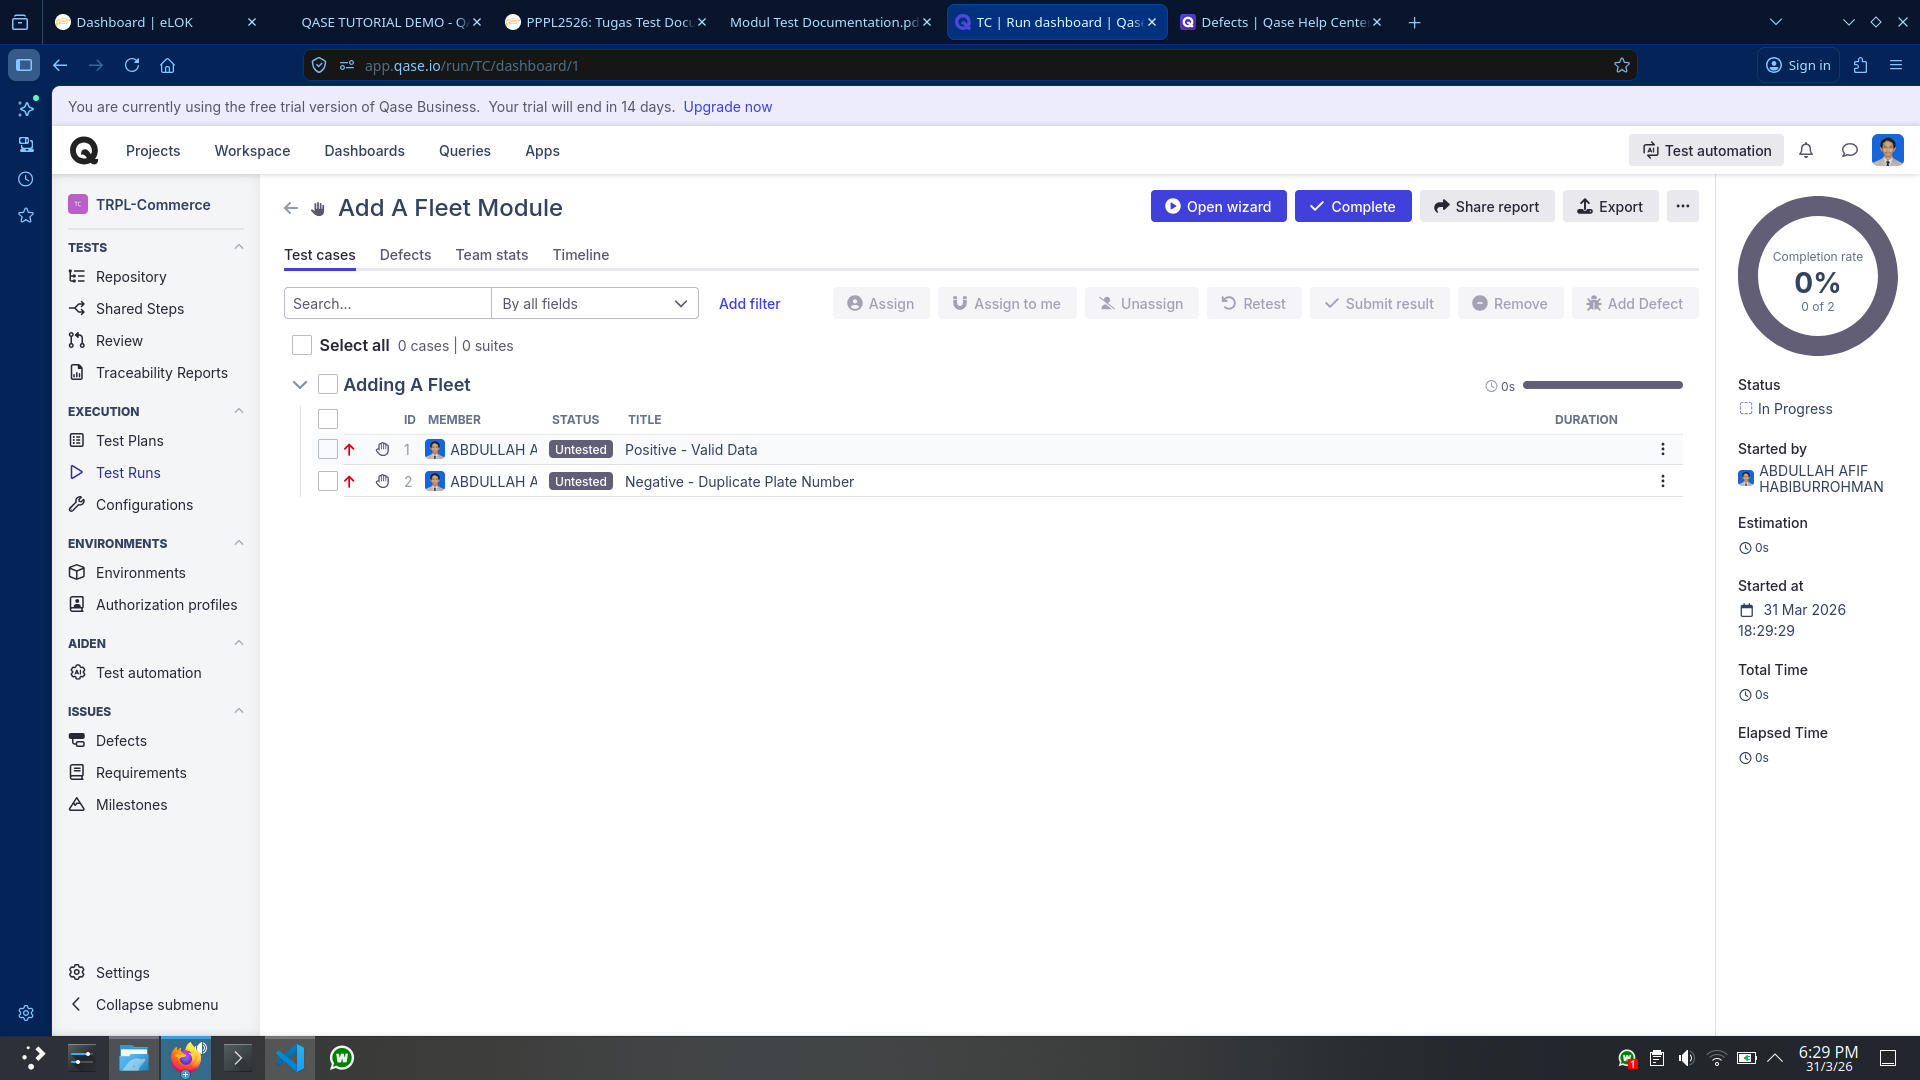
\includegraphics[width=0.8\textwidth]{Screenshot_20260331_182951.png}
    \caption{Setelah menekan tombol "Start run"}
    \label{fig:test_run1}
\end{figure}

Setelah itu, mahasiswa melakukan pengujian pada code. Kemudian karena pengujian dilakukan secara manual, mahasiswa perlu menambahkan status secara manual dengan menekan baris test case dan memilih status yang sesuai. Berikut adalah gambar langkah-langkah yang dilakukan:

\begin{figure}[H]
    \centering
    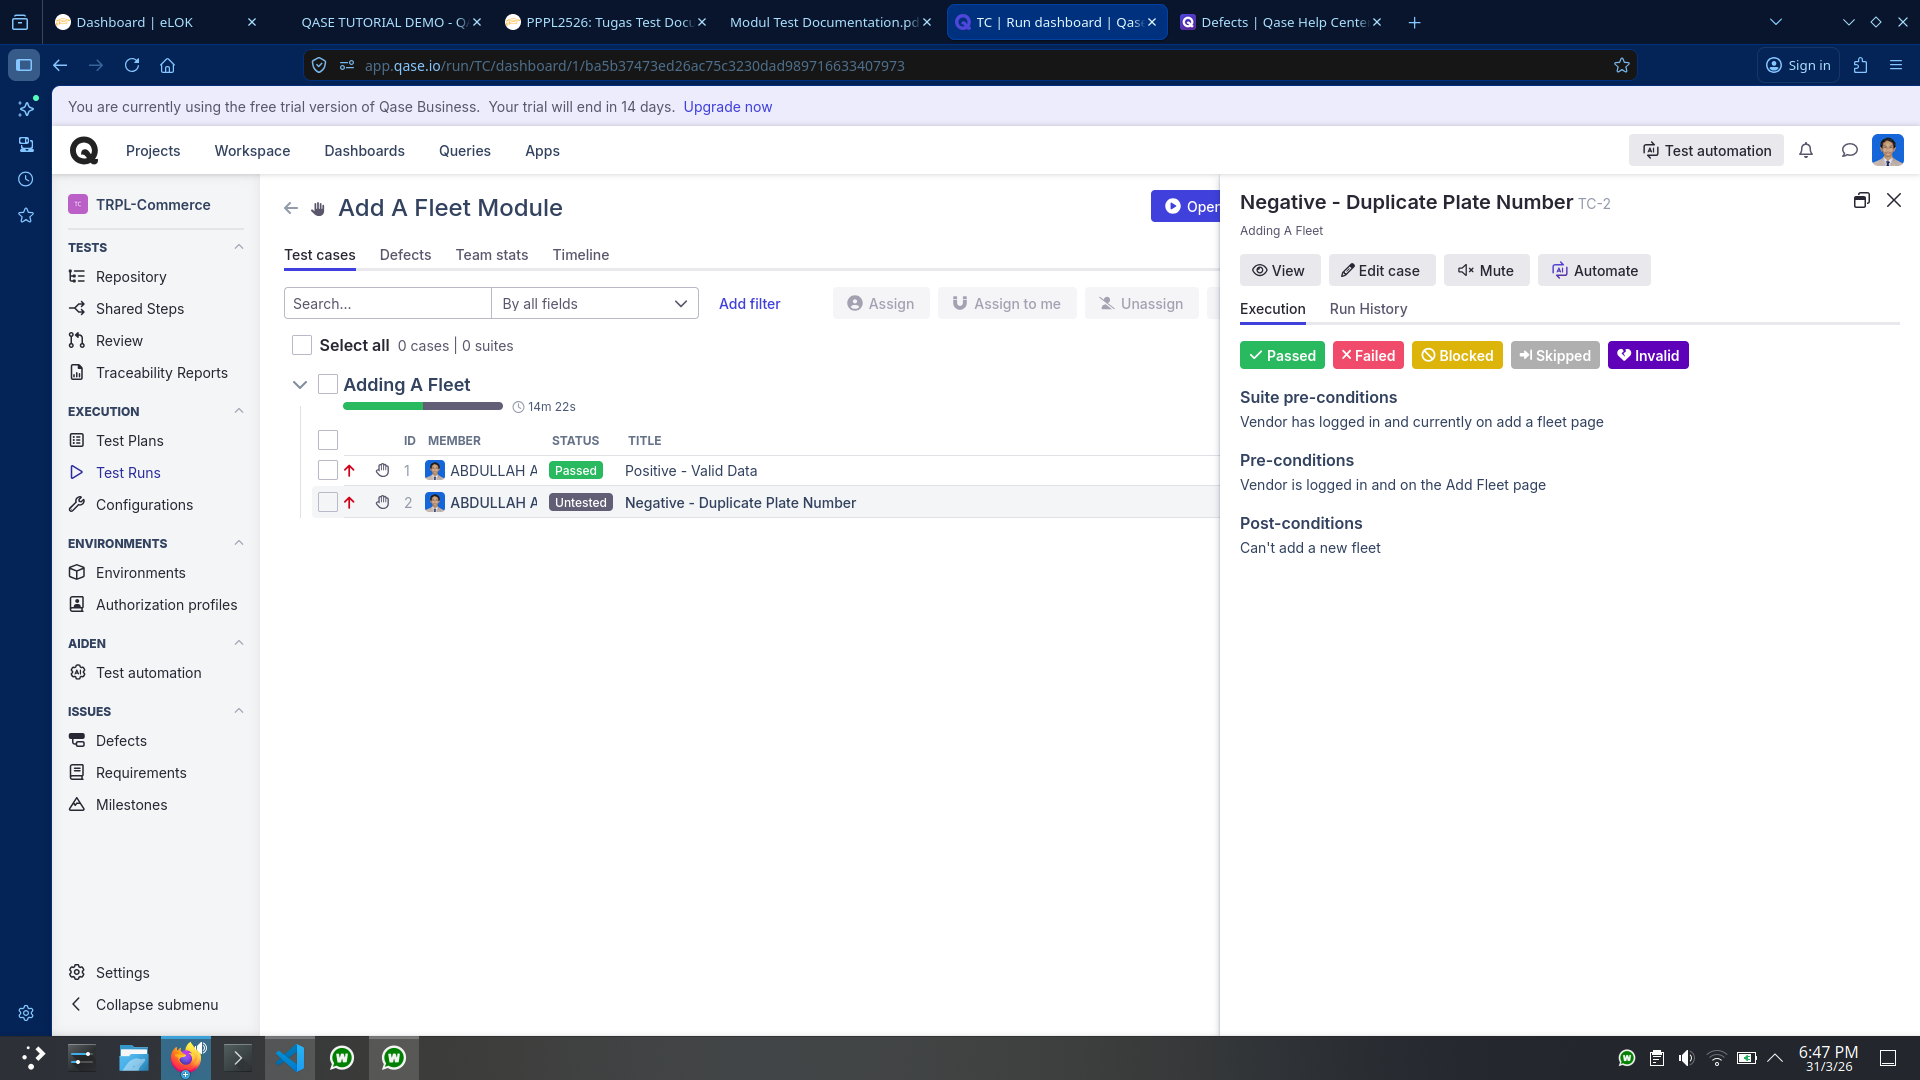
\includegraphics[width=0.8\textwidth]{Screenshot_20260331_184733.png}
    \caption{Menambahkan status secara manual}
    \label{fig:test_run2}
\end{figure}

\subsection{Bug Reporting}

Ternyata, terdapat bug pada case "Negative - Invalid Data". Hal ini disebabkan oleh data yang duplikat dapat terinput ke sistem. Seharusnya perilaku tersebut tidak terjadi. Mahasiswa kemudian melakukan report bug pada case tersebut. Berikut adalah tampilan bug report yang mahasiswa buat:

\begin{figure}[H]
    \centering
    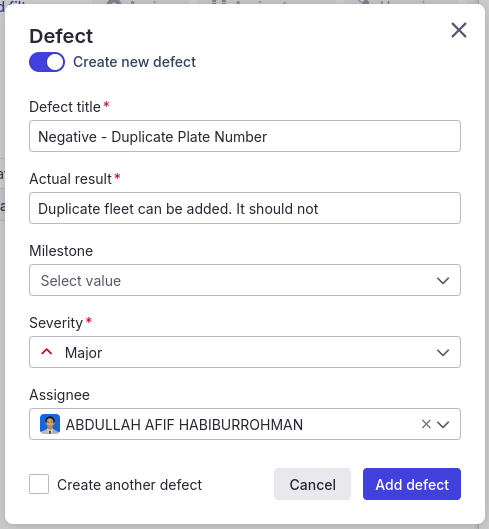
\includegraphics[width=0.8\textwidth]{fail.png}
    \caption{Pengisian Data Bug Report}
    \label{fig:bug_report}
\end{figure}

\begin{figure}[H]
    \centering
    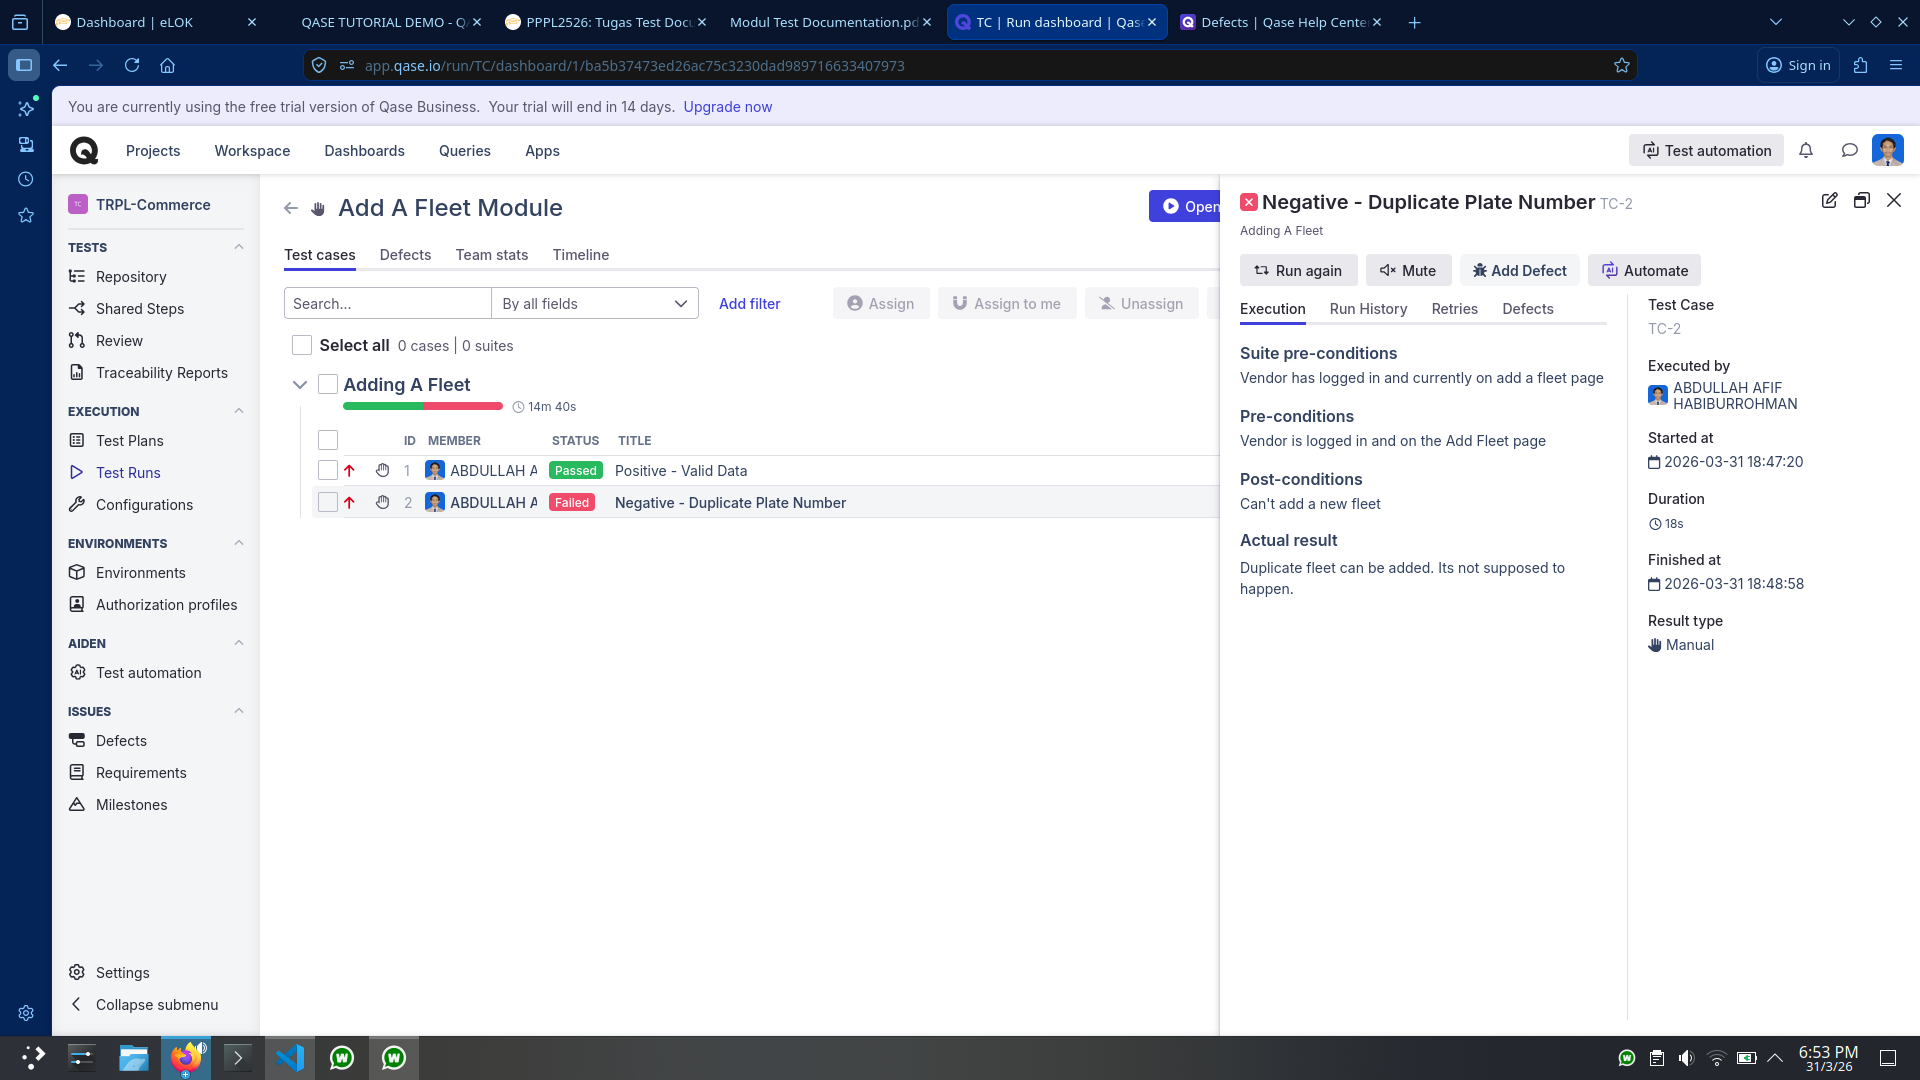
\includegraphics[width=0.8\textwidth]{Screenshot_20260331_185331.png}
    \caption{Bug Report}
    \label{fig:bug_report1}
\end{figure}

Setelah melakukan reporting, mahasiswa sudah melakukan semua testing yang diperlukan. Mahasiswa dapat melihat hasil testing dan bug report pada halaman Run Dashboard. Berikut adalah gambar dari halaman Run Dashboard:

\begin{figure}[H]
    \centering
    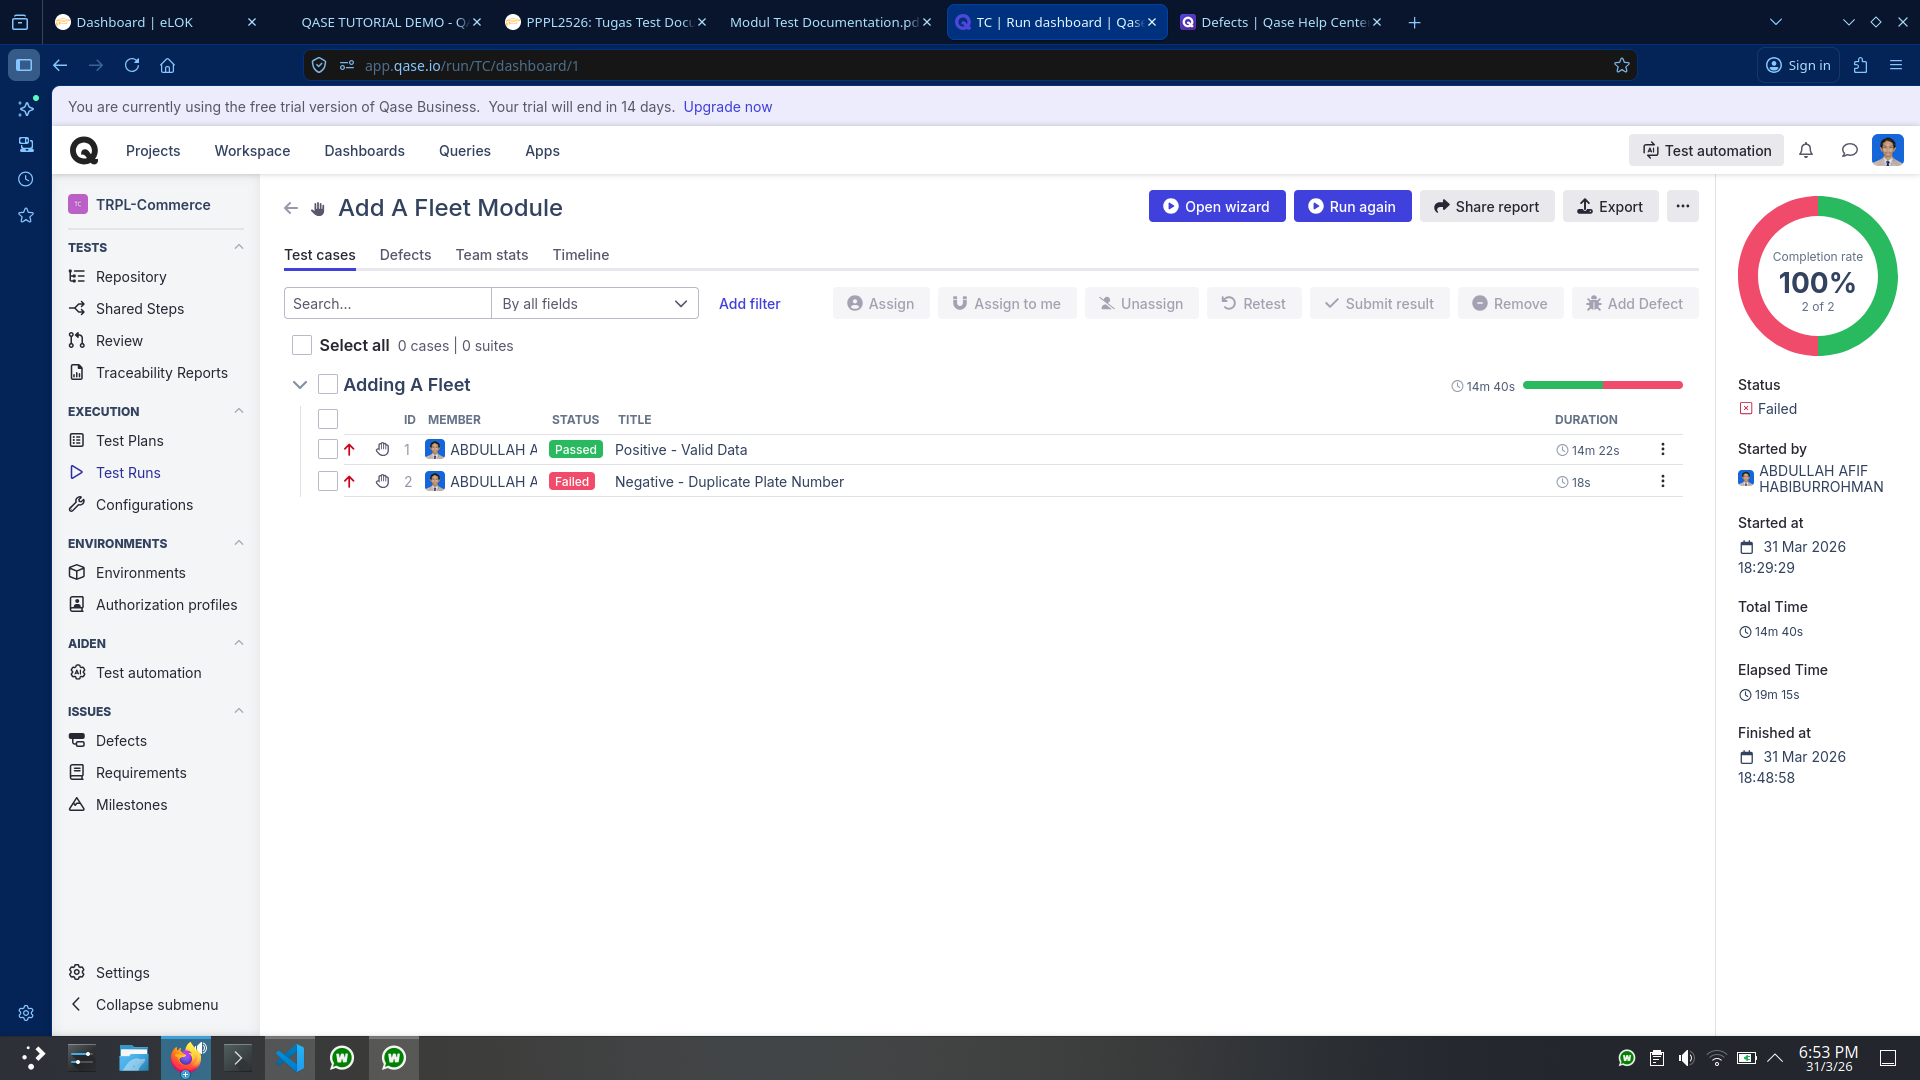
\includegraphics[width=0.8\textwidth]{Screenshot_20260331_185355.png}
    \caption{Run Dashboard 100\% Complete}
    \label{fig:run_dashboard}
\end{figure}

Berikut adalah gambar dari halaman test case yang terdapat bug:

\begin{figure}[H]
    \centering
    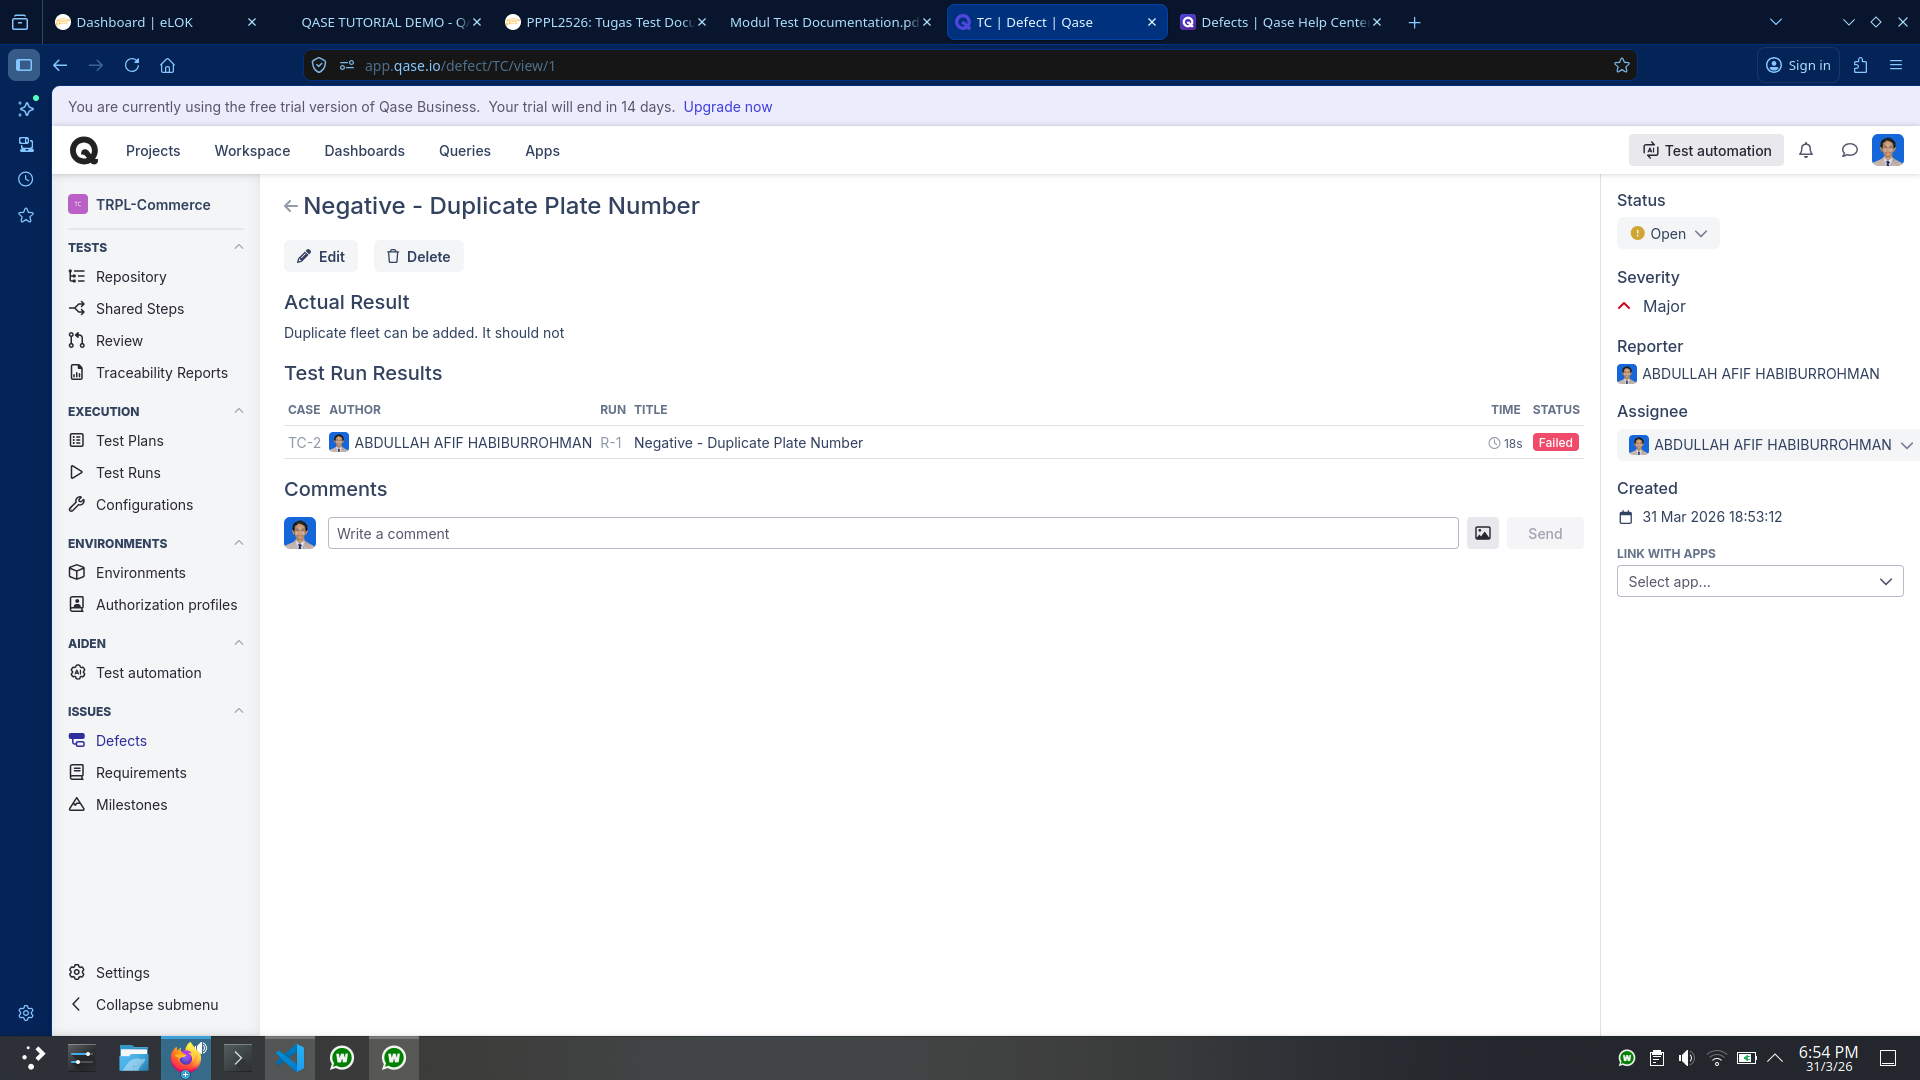
\includegraphics[width=0.8\textwidth]{Screenshot_20260331_185418.png}
    \caption{Test Case dengan Bug}
    \label{fig:test_case_bug}
\end{figure}

\end{document}